%\usepackage{graphics}

%--------------------------------------------------------------------------------------------------------------------
%------------------------------------------------- Chapter 7 --------------------------------------------------------
\chapter{Implementaciones del framework DHD: Casos de
usos}\label{cap:implementaciones} \label{cap:7}
%\pagenumbering{arabic}

\section{Introducción}

\textcolor{red}{Completa ...}

\section{Usos de los contratos sensibles al contexto: Evidencias en el uso de entornos E-learning}

A medida que el avance en la investigación y desarrollo de plataformas
e-learning brinden  mejoras e innovaciones de herramientas (videoconferencias,
porfolios, wikis, workshops, etc.) y sus respectivos servicios,  crece la
cantidad de posibles configuraciones de los espacios e-learning.  Abarcando
diferentes tipos de requerimientos pertenecientes a las etapas de diseño, otros
durante el desarrollo y otros en tiempo de ejecución. A partir de estos se
definen los procesos e-learning (Pe-lrn). Al igual que los procesos de negocios
en una Aplicación Web convencional (ej., www.ebay.com), los Pe-lrn están
compuesto por transacciones Web \cite{transaccion web}. En este contexto, una
transacción (o transacción e-learning) es definida como una secuencias de
actividades que el usuario ejecuta a través de una Aplicación E-learning con el
propósito de efectuar una tarea o concretar un objetivo. El conjunto de
actividades, sus propiedades y las reglas que gobiernan sus ejecuciones
dependen del Pe-lrn que la Aplicación debe brindar.

Las características tecnológica de un Aplicación Web e-learning (AWe-lrn) son
idénticas alas Aplicaciones E-learning convencionales (por ejemplo, las
utilizadas en el proyecto de e-learning Sakai \footnote{SaKai: Entorno
colaborativo y de aprendizaje para enseñar. Es de código abierto y está resuelto
con tecnología Java. Url: wwww.sakaiprojet.org}) 


que proveen:  navegación entrepáginas a través de links, ejecución de Transacciones  e-learning por medio de los servicios de las herramientas y las operaciones de un Pe-lrn. La principal diferencia tecnológica entre un AWe-lrn y una Aplicación e-learning convencional está en la incorporación de la teoría de coordinación de contratos \cite{fiadeiro,libro5} en la implementación de algunos servicios que las herramientas brindan a los usuarios \cite{libro}.

En base a la incorporación de los contratos en la implementación y diseño de Transacciones e-learning, aumenta las posibles configuraciones de los Pe-lrn. Comienzan a aparecer nuevas propiedades que  tienen que ver con el campo de la Ingeniería de Software. Y, a su vez,  fuertemente relacionados al trabajo multidisciplinario entre los actores de un proyecto de construcción de una AWe-lrn (ej. el proyecto Obra Abierta \footnote{Obra Abierta: Proyecto de I&D (CONICET), que se centra en el desarrollo e implementación de dispositivos hipermediales context-aware dinámico para investigar y aprender en contextos físicos-virtuales de educación superior. Directora: Patricia San Martín }). Para este fin, es imprescindible contar con un modelo de diseño que ayude en el ciclo de vida del desarrollo y configuración de una Aplicación e-learning. Integrando las tareas de los expertos en educación, diseñadores y desarrolladores. 

Desatender o resolver incorrectamente la documentación para el diseño de
procesos tipo Pe-lrn pueden causar numerosos problemas reflejados en el proceso
de configuración  de un AWe-lrn. Estos problemas pueden ser: (1) Dificultades en
la comunicación y entendimiento entre los clientes y diseñadores expertos en
educación (primero), y entre los diseñadores y los desarrolladores (después), en
el proceso de implementación de un AWe-lrn. (2) Determinación de las relaciones
donde se justifique la inclusión de contratos. (3) Dificultad para visualizar la
trazabilidad entre los procesos e-learning y las implementaciones de las
Transacciones.

Este trabajo presenta un diseño compresivo para el modelado de los procesos de
educación e-learning (Pe-lrn) en un Aplicación Web E-learning con la inclusión
de los contrato con propiedades context-aware \cite{libro}. El modelo está
basado en UWAT+ (Distante, 2004), una versión extendida y adaptada de "UWA
Transaction Design Model" para el diseño de transacciones en aplicaciones Web.
La principales contribuciones de este trabajo son: - El acercamiento de un
modelo útil para la representación de transacciones e-learning en una AWe-lrn;
permitiendo una mejor distinción de la ubicación (entre servicio-usuario(s) y
servicio-servicio(s)) de la componente contrato dentro del flujo de ejecución. -
Ejemplificar, mediante un caso de uso concreto,  el uso del modelo UWATc+.


El resto de este trabajo se encuentra organizado de la siguiente manera: Tras
esta introducción se presenta una referencia conceptual del los contratos,
utilizados en el proyecto Obra Abierta (Sección \ref{contrato}). Luego se
continúo con definiciones, formas de documentación y representación de
Transacciones e-learning y procesos. (sección \ref{documentacion}). Siguiendo,
se presenta un modelo conceptual y de diseño sobre la adaptación propuesta para
el modelado de Pe-lrn (sección \ref{uwatc}). Mediante un caso de uso concreto,
se describe el uso de UWATc+ para cada una de sus etapas. Finalizando con una
breve conclusión.


\subsection{Contratos context-Aware para transacciones en los DHD} \label{contrato7}

En términos generales, la coordinación de contratos es una conexión establecida
entre un grupo de objetos (en nuestras consideraciones, un objeto cliente y un
determinado servicio). Cuando un objeto cliente (ej. un usuario alumno) efectúa
una llamada a un objeto suministro (ej. un servicio de la herramienta Foro), el
contrato "intercepta" la llamada y establece una nueva relación teniendo en
cuenta el contexto del objeto cliente, el del objeto servidor, e información
relevante adquirida y representada como contexto del entorno. Como condición
necesaria, la implementación de los contratos no debe alterar el diseño y
funcionalidad en la implementación de los objetos.


\subsubsection {Elementos de la componente contrato}

El contrato puede ser configurado por medio de diferentes mecanismos, desde el
lenguaje cotidiano hasta un lenguaje de especificación formal y un lenguaje
basado en XML para los casos que sean necesarias especificaciones que puedan ser
procesadas por máquinas. 

El tipo de tecnología y forma de implementación de los contratos es transparente
para los objetos que consumen los servicios en donde se encuentran involucrados.
La configuración de un elemento contrato que forma parte de  las componentes de
un servicio, representa la información necesaria del mismo para ser utilizado
por el invocador, sin necesidad que el dicho objeto tenga detalles de la
ejecución.
El contrato representa una enriquecida y efectiva interface de construcción que
contiene toda la información sobre las componentes de los servicios, y deberá
tener referencias sobre algún tipo de información de contexto para su
utilización.

En la figura \ref{contratoca} se puede observar los elementos conceptuales
básicos de esta componente a través de una serie de elementos que lo relacionan.

\begin{figure}[!h]
\begin{center}
		
		\begin{center}
 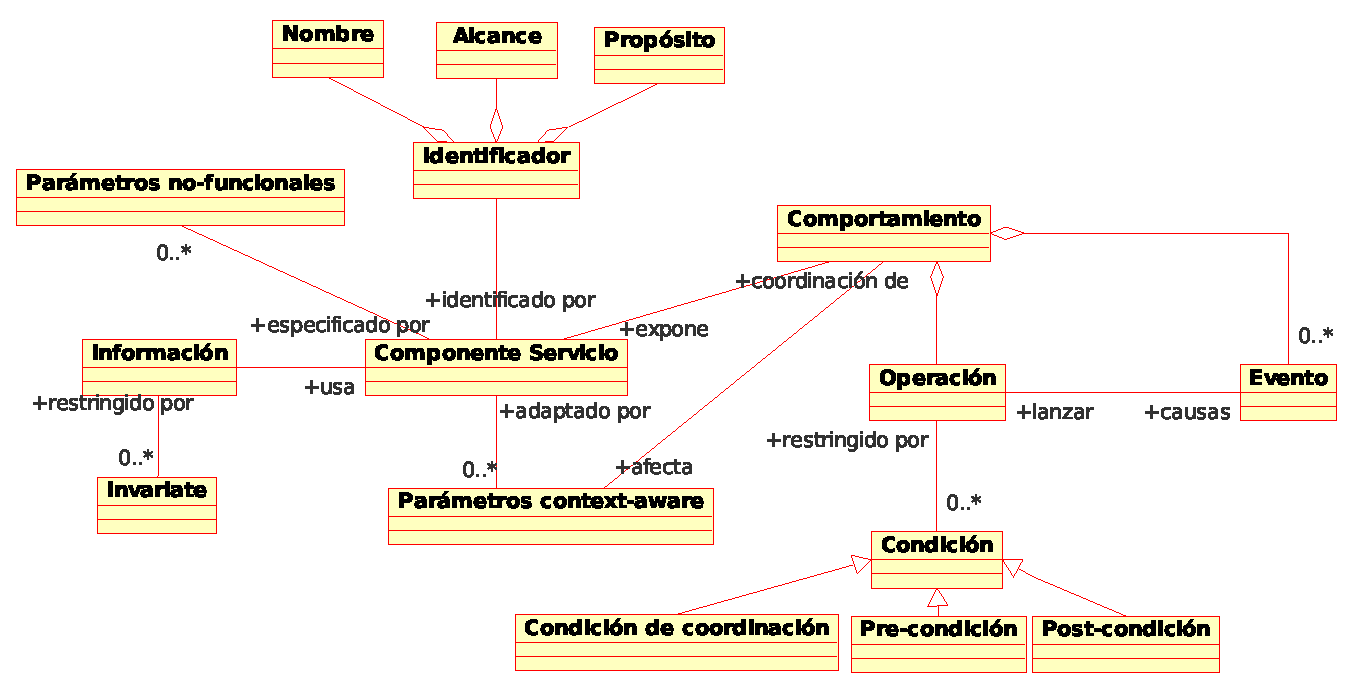
\includegraphics[width=6 in,totalheight=2.4 in]{Ch7/contratoca}
 % procesodiseno.png: 435x165 pixel, 90dpi, 12.28x4.66 cm, bb=0 0 348 132
  \caption{..}\label{}
\end{center}
\end{center}
\end{figure}
 
 


Para una mejor comprensión de las componentes del modelo se explica su
caracterización y funciones particulares: 

\textit{Identificador} – Una componente servicio es identificada para un
determinado contexto por un único nombre en el espacio de nombre.

\textit{Comportamiento} -  De acuerdo con los roles asignados en un determinado
contexto, una componente servicio expone comportamientos correspondientes a la
provisión y pedido de operaciones, y/o publicaciones y recepción  desde/hacia
cada contexto. Las operaciones pueden ser definidas en dos tipos – operaciones
que ejecutan cómputos o transformaciones (tipo “update”) y operaciones que
proveen algún tipo de información sobre consultas  (tipo “query”). Estas, se
encuentran enteramente especificadas en base a  un contrato, con el uso de
pre-condición, post-condición y condicionales para lograr la coordinación entre
contratos. En las condiciones de coordinación se especifican cómo requerir y
proveer operaciones. Para lograr una comunicación precisa con una componente
servicio, no sólo se tiene en cuenta qué operación fue provista o requerida y
cómo el ejecutor ha lanzado el evento apropiado, sino también, cómo todas esas
actividades están mutuamente relacionadas para ser aprovechadas por el objeto
cliente. Un evento del contexto que lanza una operación dada, puede ser parte de
un conjunto de pre-condición, mientras que un evento emitido a través de una
operación exitosa puede ser parte de una pos-condición. 

\textit{Tipos de Información} –  Una componente de servicio debe  manejar, usar,
 crear o tener cierta información de recursos con el propósito de proveer
servicios adecuadamente.  Este elemento del contrato define el tipo de
información relevante para las componentes  asociadas al contrato, así como
también restricciones y reglas sobre instancias de esos tipos. Esto representa
un modelo de información lógica de una componente de servicio. Formalmente, esta
información de tipos puede ser considerada como definiciones de tipos de  los
parámetros de las operaciones, o tipos relacionados a ellos.

\textit{Configuración de Parámetros Context-Aware} – Una componente servicio
depende del contexto de su actual entorno. Para utilizarse en diferentes
contextos logrando la adaptación a eventuales cambios debe tener definido un
conjunto de parámetros de configuración.  Ejemplos de estos parámetros pueden
ser: Contexto-del-Usuario (CU), locación en tiempo y espacio de los servicios
consumidos y suministrados. Estos parámetros pueden ser enviados dentro de las
invocaciones de las operaciones de los servicios o por medio de otros caminos,
mediante componentes de servicios que pueden adaptar su comportamiento ante el
cambio de contexto en una determinada situación.  

\textit{Parámetros no funcionales} – Una componente servicio puede definir un
conjunto de los llamados parámetros no funcionales que caracterizan a la
“calidad” de sus prestaciones dentro de un determinado contexto. Estos
parámetros, son elementos para los consumidores de los servicios que permiten
optar por el uso de un determinado  servicio, o buscar otro con el mismo o
similar contrato. Como ejemplo de parámetros no funcionales podemos mencionar:
Performance, Fiabilidad, Tolerancia a Fallos, Costos, Prioridad y Seguridad.


\subsection{Documentación de los DHD procesos} \label{documentacion7}

Las transacciones e-learning en un AWe-lrn están definidas como secuencias de
actividades asociadas con un flujo de ejecución que permite al usuario
desempeñar una determinada tarea  y/o alcanzar una meta a través de la
Aplicación. Entonces, un proceso e-learning (Pe-lrn) puede ser interpretada como
una especificación del concepto de "workflow" en una Aplicación e-learning Web,
con las condiciones (restricciones) que implica su concreción. En una
Transacción e-learning Web, una  $Actividad$ está  conformada por un conjunto de
operaciones simples o complejas sobre datos y contenidos de la Aplicación. Como
ejemplo de Transacciones e-learning se pueden mencionar un proceso en el cual un
usuario (alumno) participa en un espacio de edición colaborativa (este caso será
analizado posteriormente como caso de uso en las secciones posteriores) 

Entonces, las transacciones en un AWe-lrn son el camino para la representación
de los Pe-lrn, y proveer a los usuarios de servicios accederlos por medio de las
herramientas que los contienen (wiki, foro, vídeo conferencia, taller, blog,
etc.) La ejecución de Transacciones de un AWe-lrn supone tanto la navegación a
través de las herramientas, por medios de los links de las componentes
hipermediales, como  el uso de sus servicios. Un ejemplo de servicio puede ser
en una vídeo conferencia la posibilidad de que un docente edite en una pizarra
compartida (con sus alumnos y colaboradores) una determinada ponencia. 

El diseño de las transacciones abarca varios niveles de abstracción, distintos
formalismos pueden ser usados para su representación y documentación. Al menos
tres niveles de abstracción pueden ser representados: (1) nivel conceptual, (2)
nivel lógico, y (3) nivel de implementación.  El diseño conceptual permite una
representación del sistema (las transacciones y su alcances) tal cual son
"percibidas" por el usuario y despejando las cuestiones de implementación. El
diseño de la implementación se encuentra focalizado a proveer a los diseñadores
de los AWe-lrn con todas las especificaciones necesarias para la configuración y
realización de sus componentes. El diseño lógico es un nivel intermedio del
diseño de abstracción, utilizado para  trasladar las especificaciones centrales
del usuario desde el diseño conceptual hacia términos de  especificaciones más
cercana a las implementaciones.


Al igual que lo que ocurre con todos lo artefactos de software, el diseño de una
Transacción e-learning para un AWe-lrn  se puede tornar muy complejo. Cuanto más
complejo sea el diseño, las confusiones entre los diseñadores (expertos en
educación y analistas informáticos) y los implementadores (programadores y 
encargados de la Aplicación) crecerán. Para comunicar efectivamente la idea del
diseñador es necesario una apropiada documentación. Si bien la documentación
textual ha sido muy utilizada para describir detalles de implementaciones de
bajo nivel, teniendo en cuenta que el diseño de las transacciones e-learning se
describen en un  nivel conceptual, es más adecuado una representación gráfica. 

Existen diferentes aportes  directamente relacionado a modelos "visuales" en
forma de documentación gráfica \cite{5,10,12}. En este contexto los modelos
visuales son representaciones de sistemas de software que soportan múltiples
perspectivas. Para el caso del diseño de las transacciones e-learning, una vista
puede ser representada por una series de diagramas pertenecientes a UML (Unified
Modeling Language) \cite{UML} 

Los antecedentes relevantes que se relacionan con lo que entendemos por diseño
de Pe-lrn, fueron estudiados de los aportes en el campo de los métodos de
diseños para Aplicaciones Web experimentados en los últimos años. Concretamente
se pueden mencionar ADM (Atzeni y Parente, 2001), OO-H (Koch et al., 2003),
OOHDM (Schmid - Rossi, 2004) y UWAT+ (Distante, 2005).

UWAT+ es un meta-modelo para la descripción de los distintos aspectos de
Transacciones Web de manera holística. Es una extensión del Modelo de Diseño de
Transacciones que forma  parte del framework UWA (Ubiquitous Web Applications)
\cite{UWA}. Inspirado en este modelo y extendiéndolo para la contención de los
contratos, se describe una adaptación para el diseño de Transacciones e-learning
en un AWe-lrn.

\subsection {UWATc+: una adaptación de UWAT+ para el modelado de DHD procesos } \label{uwatc7}

Si bien los métodos de diseño de Transacciones de UWAT+ pueden ser utilizados
para la representación de Transacciones e-learning, es necesario efectuar
adecuaciones que tengan en cuenta la inclusión a los contratos (según sección
\ref{contrato}). Tal cual fue mencionado en la sección \ref{intro}, desde la
perspectiva de los diseñadores, los contratos deben ser visto como una pieza de
software para la instrumentación de los servicios de las herramientas. En
consecuencia, es necesario tener un modelo que permita una mejor representación
de los contratos, la visualización de su inserción en los servicios y las
relaciones que en ellos representan (relaciones entre objetos que implementan
servicios, usuarios y herramientas en la Aplicación). 


La figura \ref{drobab} se muestra un diagrama de clase UML que representa a los
conceptos, las relaciones entre conceptos y los modelos para la representación
de Transacciones. Los esquemas en color blanco pertenecen al modelo original
UWAT+. El rectángulo y los esquemas grises describen los objetos, modelos y
relaciones que  que conforman el nuevo modelo denominado UWATc+.

	\begin{figure}[!h]
        \begin{center}
        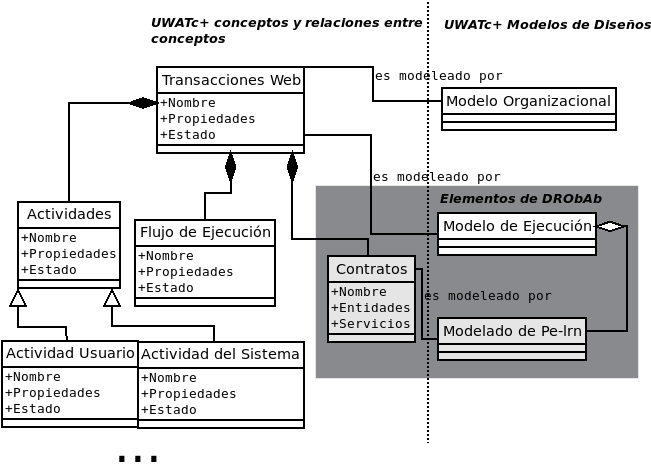
\includegraphics[width=5.3 in,totalheight=3.3 in]{Ch7/drobab11.png}
	\caption{\small \sl UWATc+ modelo conceptual y de diseño} \label{drobab7}
         \end{center}
         \end{figure}


Como se describe en el diagrama, una Transacción Web es un objeto complejo
(conceptual) compuestos por dos tipos de objetos principales pertenecientes al
modelo original de UWAT+ y un tercer objeto  agregado para la representación de
los contratos pertenecientes a las Transacciones e-learning. En el primer grupo
se encuentra $Actividad$ para la distinción de las actividades de los usuarios y
del sistema. El objeto $Flujo de Ejecución$ representa el orden lógico y
temporal para la ejecución de las actividades comprendidas en las Transacciones.
A su vez, una Transacción Web puede ser descripta por el $Modelo Organizacional$
(desde el punto de vista estático) y el $Modelo de Ejecución$ para la definición
de las reglas de ejecución de la componente actividad (desde el punto de vista
dinámico). 

Cuando una Transacción Web contiene un contrato (definida como transacción
e-learning) debe ser incluida una nueva componente para el diseño (representada
en la figura como una relación de agregación en el $Modelo de Ejecución$),
conjuntamente con un nuevo modelo de diseño, $Modelo de Pe-lrn$, que permitirá
la representación del contrato (caracterizada como relación de asociación con el
objeto $Contrato$).

De esta manera quedan conformados los elementos que componen el modelo UWATc+
(rectángulo gris) y sus relaciones con el modelo original UWAT+. A continuación
se describe, en detalle, el modelo usado por UWATc+ para el diseño de los
transacciones que utilizan contratos (transacciones e-learning). 


\subsubsection{Requerimientos para el diseño de DHD Transacciones}

En esta sección se describen la caracterización de dos tipos representativo de
requerimiento que motivaron la creación de este nuevo modelo de diseño
(definidos en la sección \ref{intro}). En base a experiencias recogidas por el
grupo del proyecto Obra Abierta en el diseño y configuración de Aplicaciones
e-learning, se presentarán dos tipos de requerimientos que deben ser cubiertos
por el modelo de diseño. En primer lugar se enuncian cuestiones técnicas de
diseño (desde el punto de vista de la Ingeniería de Software), seguido de un
comentario sobre el tipo de Transacciones que el diseñador puede especificar a
través del modelo.

\begin{itemize}

\item Especificar como son afectadas la ejecución de las actividades por los
objetos contratos. 


La relación de una actividad con un contrato se produce cuando existen objetos
interrelacionados por medio de un contrato \cite{fiadeiro}. De esta manera, el
diseñador debe poder documentar las información de los objetos involucrados, sus
métodos y parámetros. El contrato representa un tipo diferente de relación a la
original entre los objetos, con la propiedad de reconfiguración en tiempo de
ejecución. Característica que permiten una mejor adaptación a los requerimientos
que resuelven las Transacciones e-learning.

\item  Definir cuál y cómo la  información de los objetos contratos
("information object" \cite{informationobject}) es afectada por la ejecución de
las Actividades.


Una actividad funcional consiste en la ejecución de uno a más operaciones
elementales (inserción, borrado, modificación, etc.) sobre los datos de la
Aplicación y la información de los objetos contratos envuelta en la Actividad.
El modelo de diseño de Transacciones e-learning debe permitir al diseñador
definir cuales operaciones del contrato son fundamentales para cada actividad,
modelando el camino en que cada actividad elemental afecta la información de los
objetos involucrados (modificando sus instancias por medios de sus ejecuciones).
\end{itemize}


\subsection {Diseño de procesos e-learning con UWATc+} \label{diseno7}

En esta sección se describen los resultados de la Aplicación de UWATc+ para el
espacio dedicado al libro "Hacia un dispositivo hipermedial context-aware
Dinámico. Educación e investigación para el campo audiovisual interactivo" (San
Martín P. 2007, et. al) \cite{libro}.  Este  modelo fue aplicado parcialmente
para el diseño de los requerimientos fundamentales y el modelado del
comportamiento funcional enmarcado bajo la perspectiva de proyecto Obra Abierta
- mencionado anteriormente. Se presentará un caso de uso para ejemplificar el
diseño de un Pe-lrn en la Aplicación e-learning para Obra Abierta. El diseño
describe parte del proceso en que un usuario hace uso de los servicios de
edición de la herramienta Foro a través de un contrato. 

	\begin{figure}[!h]
        \begin{center}
	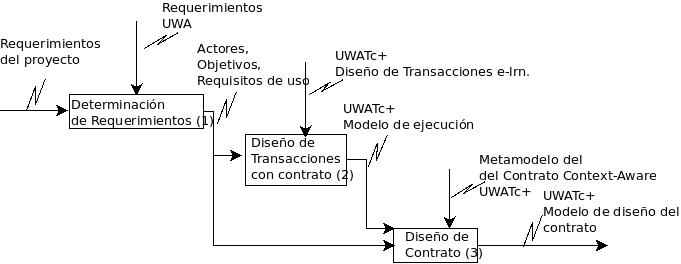
\includegraphics[width=6 in,totalheight=2.5 in]{Ch7/procesodisenoNuevo.jpeg}
	\caption{\small \sl El proceso de diseñar Pe-lrn en un AWe-lrn con UWATc+} \label{procesodediseno7}
         \end{center}
         \end{figure}



El diagrama de la figura \ref{procesodediseno} muestra una adaptación del diseño
de procesos de UWA \cite{UWA} que se utiliza en UWATc+ para el diseño de
transacciones con contratos. Para ilustrar el proceso de diseño se utiliza la
notación IDEF0 (IDEF-0, 1993). En comparación con la metodología original de
UWAT+, se agregaron las fases del diseño de contrato y fue modificado el modelo
de diseño de la transacciones. Además, fueron excluidas las fases de "diseño de
la información" y "diseño de publicación". Las fases del proceso de diseño
quedan conformadas de la siguiente manera: (1) Determinación de Requerimientos;
(2) Diseño de transacciones con contrato; (3) Diseño de contrato.

\subsubsection{Determinación de Requerimientos} \label{sdr7}

La fase de Determinación de Requerimientos toma como entrada las
especificaciones del proyecto y produce, por medio de un mecanismo de
refinamiento, las siguientes salidas: Cada actor con su objetivos relativo. Los
requerimientos para la construcción y configuración de un AWe-lrn.
 
El modelo utilizado es orientado a objetivos: cada actor se identifica con al
menos un objetivo, i.e, una abstracción de los objetivos que a través de la
aplicación se debe alcanzar; cada objetivo es refinado en otros sub-objetivos,
hasta poder definir el requerimiento en un bajo nivel suficiente para poder ser
implementado. Este fase es similar a la descripta en (UWA Consortium, 2001)
\cite{UWA}. 

	\begin{figure}[!h]
        	\begin{center}
		 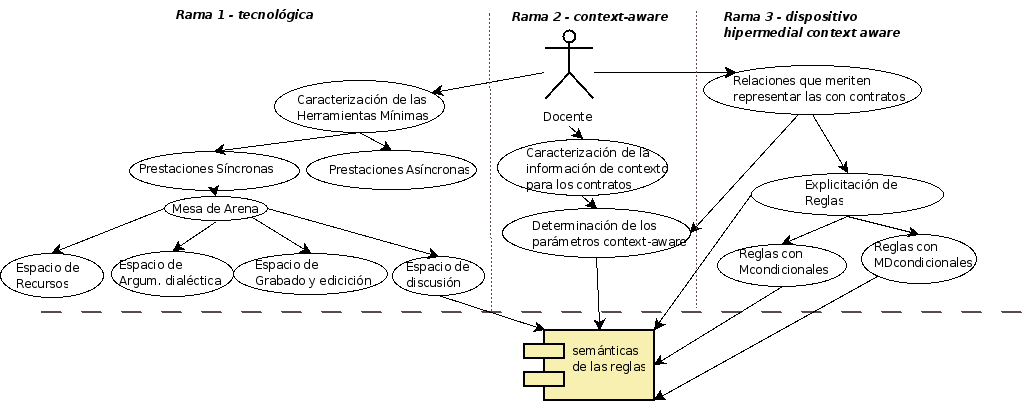
\includegraphics[width= 5 in,totalheight=3.8 in]{Ch7/Requerimientos}
                \caption{\small \sl Objetivos de al alto nivel para un Pe-lrn}
\label{requerimientos7}
         	\end{center}
         \end{figure}

Para este caso de uso, atendiendo a los lineamientos en \cite{libro}, se
describe parte del modelo original donde se caracterizan los objetivos
involucrado con un actor del sistema. A su vez, a medida que se van derivando
los sub-objetivos comienzan a establecerse requerimientos concernientes a la
teoría de coordinación de contratos context-aware \cite{libro5,fiadeiro}. En la
figura \ref{requerimientos} dicha situación ocurre en la derivación de las tres
ramas de objetivos y sub-objetivos, influyendo directamente en la composición de
la componente contrato. En este caso, tomando desde la \textit{\textbf{rama 1}}
un servicio de una herramienta de un espacio de discusión (herramienta Foro); de
la \textit{\textbf{rama 2}} se desprenden la información necesaria para poder
articular dicho servicio teniendo en cuenta la información de contexto;  la
\textit{\textbf{rama 3}} aporta el consenso de los expertos (del dominio
e-learning) para la inclusión de los contratos en aquellas relaciones que
mantendrán las propiedades de la Aplicación e-learning \cite{libro5}. A través
de este modelo, se logra un primer acercamiento sobre como se relaciona un
contrato con: los requerimientos, el tipo de objetivos para cada requerimiento y
los actores del sistema. 

\subsubsection{Diseño de DHD-Transacciones}

El diseño de transacciones e-learning retoma la misma idea y modelo propuesto
por UWAT+ para el diseño de transacciones \cite{UWAT}. Partiendo de los
resultados de la fase de \textit{Determinación de Requerimientos},
fundamentalmente de la caracterización de los contratos, pueden ser
seleccionados una series de transacciones, i.e., objetivos que requieran la
ejecución de una o más Actividades para su cumplido. Para cada uno de los
objetivos que incluya contrato deben ser diseñadas Transacciones e-learning (de
igual forma que con las transacciones en UWAT+), los cuales en principio deben
ser establecidos desde un punto de vista estático (en este trabajo no
abordaremos tal consideración) y luego, desde un punto de vista dinámico por
medio de un modelo de ejecución. En la figura \ref{modelodeejecucion} se muestra
una porción del modelo de ejecución de un transacción e-learning cuyo contrato
asociado fue caracterizado en la fase de \textit{Determinación de
Requerimientos} (figura \ref{requerimientos}, sección \ref{sdr}). En el diseño
se describe el flujo de ejecución entre las Actividades de la transacción. El
modelo de ejecución es una adaptación del diagrama de actividades de UML
\cite{7} en el que las Actividades y sub-Actividades están representadas por
estados (óvalos), y el flujo de ejecución entre ellos se representa por medio de
transiciones (arcos). Los óvalos con el símbolo (*) - un asterisco entre
paréntesis - refiere a una Actividad que representa a un conjunto de Actividades
compuestas, y cuyo modelo de ejecución debe ser representado con otro diagrama.
Un óvalo simple representa una Actividad Elemental. Un óvalo color gris indica
una Actividad compuesta de las sub-actividad que se encuentra dentro. Una
sub-Actividad representada con un óvalo color gris indica que es dependiente de
la Actividad que la contiene, esto quiere decir que su ejecución estará
acompañada por otra sub-Actividad y no puede ser incluida en otra composición.
Los arcos de lineas continuas indican flujos de ejecución obligatoria
(transacciones hacia Actividades requeridas), mientras que los actos con lineas
de puntos representan flujo de ejecuciones opcionales  (transacciones hacia
Actividades opcionales).
 
Cada relación posible entre actividades es representada por medio de una arco
entre ellas. A cada arco se le asocia un texto que indica bajo que condiciones
se produce la transacción, o el resultado de la ejecución de la Actividad de
origen. Para describir como colaboran los usuarios de la aplicación en la
ejecución de la Actividades puede ser anexado un diagrama UML Swimlanes. 

Cuando una Actividad ejecuta servicios implementados por contratos, entonces, se
establece un arco saliente hacia un contrato. El contrato tiene un nombre, y
entre paréntesis se indican cuales son los objetos participantes (en el caso de
tener ese tipo de información). Para representarlo visualmente se utiliza el
estereotipo del elemento componente de UML. Las Actividades que influyan en la
modificación de los contratos en tiempo de ejecución se conectan a través de un
arco de linea de puntos, igual a los utilizado en la representación de los
flujos opcionales. Los detalles de implementación del contratos se detallan en
un diagrama aparte, perteneciente a la fase descripta en la siguiente sección.

	\begin{figure}[!h]
        \begin{center}

	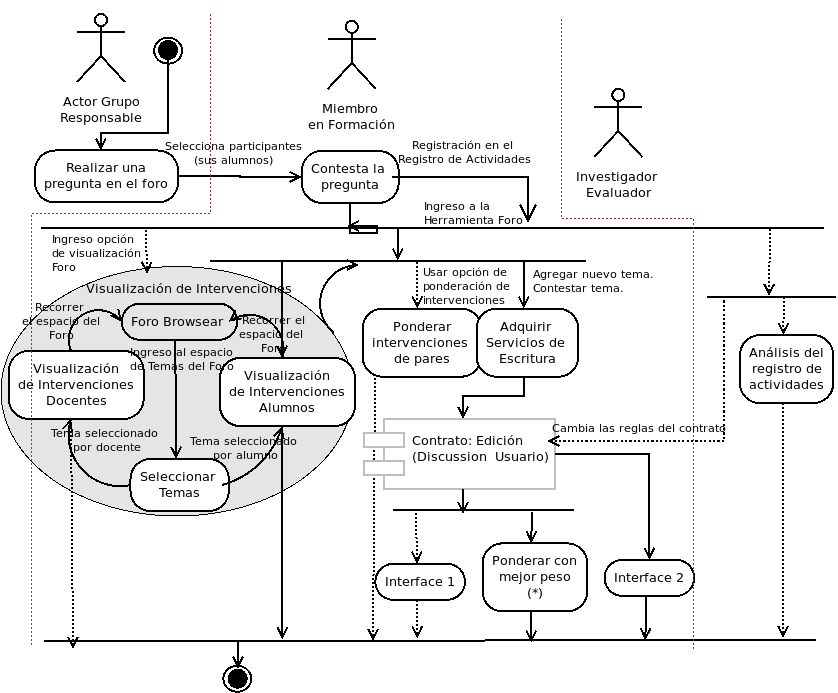
\includegraphics[width=5 in,totalheight=4 in]{Ch7/proceso11.png}
    \caption{\small \sl Modelo de ejecución de Procesos con Transacciones e-learning} \label{modelodeejecucion7}
         \end{center}
         \end{figure}


Por ejemplo, una de las opciones de la herramienta Foro de Obra Abierta
$(http://200.80.157.171:8080/portal)$ es la visualización de las intervenciones
de los usuarios en el Foro. Un usuario docente puede seleccionar la opción
"Foro" de la página principal de la Aplicación, luego seleccionar el tipo de
"vista" (mediante un "comboBox") para ingresar en modo "browser" donde se
muestran las intervenciones de los usuarios por temas. Una vez seleccionado el
tema (por medio de la Actividad "Seleccionar Tema", figura
\ref{modelodeejecucion}), es posible ingresar al espacio de las intervenciones
de los usuarios por medio de los roles de docente o alumno. Los docentes y
alumnos tienen diferentes tipos de "vistas", permisos y servicios asociados
(representadas en las actividades: "Visualización de Intervenciones Docentes" y
"Visualización de Intervenciones Alumnos"). A  través del Browser (Actividad
"Foro Browser") se recorre todo el contendido del espacio y al mismo tiempo
puede ser seleccionado otro tema para visualizar.

En cambio, si la opción seleccionado es añadir o responder temas, se ingresa a
una página Web configurada para editar texto (por medio de la Actividad
"Adquirir servicios de escritura"). Algunos de los servicios de edición y
configuración de opciones son implementadas a través del contrato "Edición"
(representado por la figura de la componente UML, con el contorno color gris).
El flujo de ejecución, luego de la intervención de los contrato, dependerán de
las reglas de coordinación y se representan con los arcos salientes similares a
los usados para representar las relaciones entre estados.


\subsubsection{Diagrama de un Contrato}

Existen diferentes formas de representación de los contratos definidos en la
sección \ref{contrato}, la herramienta  CED (Coordination Development
Environment) \footnote{CED: es el primer prototipo de una herramienta que
implementa el uso de la coordinación de contrato en aplicaciones Java. La
herramienta pertenece a ATX Sotfware (www.atxsoftware.com.ar);fue desarrollada
en Java y es de código abierta.} los implementa a través de un lenguaje llamado
Oblog \cite{lenguajeoblog}. En \cite{communit} se muestra como a través de
CommUnity se definen primitivas de modelado y técnicas de diseño basadas en la
separación de la "coordinación" del "cómputo". 

En UWATc+ se brinda un diagrama de representación de contrato, donde se
describen todos los datos que lo instancian. Cada tipo de dato y valor,
pertenece a un elemento del meta-modelo de la figura \ref{contratoca}. Teniendo
en cuenta la figura \ref{diagramacontrato}, en primer lugar (item 1) se
identifican los objetos participantes en el contrato; en el ejemplo de la figura
\ref{diagramacontrato} $DiscussionAction$ y $UserAction$ hacen referencias a dos
clases reales perteneciente a la implementación de la herramienta Foro y
Usuarios de la Aplicación Obra Abierta, respectivamente. Luego, se identifican
los nombres de los parámetros context-aware significativos para el contrato,
alineados en la misma columna del objeto que lo comparte (item 2). En Servicios
(item 3) deben ser representados los métodos del objeto, que al ser ejecutados,
provocan la intervención del contrato. Para este ejemplo $initState$ y
$getIdentifier$  son ejecutados cuando un usuario ingresa a la herramienta Foro
y las posteriores funcionalidades (servicios) disponibles  dependen de la
ejecución del contrato $Edición$ (la figura \ref{modelodeejecucion} muestra la
superposición del contrato entre los servicios de edición y las nuevas
interfaces o funcionalidades). Las siguentes filas (items 4 y 5) se refieren a
las pre y post-condiciones que se deben cumplir en la ejecución del contrato.
Por último se explicitan las reglas de coordinación. Siguiendo con el ejemplo,
en la parte del condicional $u.contexto=’l1;p1;docente;r1;c1;’$ verifica si el
contexto del usuario $u$ está compuesto por la locación $l1$, tienen el perfil
$p1$, es un $docente$, cumple el rol $r1$ y pertenece a la categoría $c1$ (este
tipo de representación de contexto se encuentra desarrollado en \cite{libro}).
En cuanto a la acción de la regla de coordinación, continuando con el mismo
ejemplo, se induce la ejecución del método $showMessage$ del objeto $d$
(DiscussionAction). El final del diagrama está dedicado a comentarios generales;
cada comentario debe ir acompañado con el número de item (1,2,3,4,5 o 6) al que
hace referencia. 

 \begin{figure}


\begin{center}

\small{ 

\begin{tabular}{|l|p{20mm}|p{55mm}|p{1mm}|p{55mm}|} 
		\hline 
\multicolumn{5}{|c|}{\textbf{Contrato:} Edición}\\
		
\hline 
1.& \textit{Participantes}: 	& \textbf{d}:DiscussionAction &&
\textbf{u}:UserAction \\
\hline 
2.& \textit{Param. c-a}: 	&	state, portlet, rundata, context &&  
context$_$identifier, identifier 	\\
3.& \textit{Servicios}:		& 	initState()		 	 &&
getIdentifier()				\\
4.& \textit{Pre-Cond}: 		& existe $<contexto>$ 			&&
existe $<contexto>$  \\
5.& \textit{Pos-Cond}: 		& modifica $<contexto>$ 		&& \\
\hline 
6.& \textit{Reglas      de Coordinación}: & \multicolumn{3}{l|}{{\textbf{Si}
\textbf{u}.contexto='p1;d;r1;c1;' \textbf{entonces}
\textbf{d}.showMessage(data,string)}}  \\
\hline 

\multicolumn{5}{|c|}{\textbf{Comentario}} \\
\multicolumn{5}{|l|}{1. DiscussionAction y  UserAction  pertenecen a clases
implementadas en JAVA del proyecto Sakai. } \\
\multicolumn{5}{|l|}{4 y 5. $<contexto>$ refiere a un objeto donde se oculta
toda la información de contexto} \\ 

\multicolumn{5}{|l|} {que caracteriza a los usuarios de la plataforma} \\



\hline
\end{tabular} 
}
\end{center}

   
	\begin{center}
	\caption{\small \sl Diagrama del contrato: Edición}
\label{diagramacontrato7}
         \end{center}
  \end{figure}



\section{Desarrollos Context Aware en el campo del sonido}


En el área de la música y del sonido, encontramos a nivel internacional, un buen número
de desarrollos donde se ha aplicado la tecnología context-awareness, realizados en el
marco de distintas universidades.
Existen en la actualidad, varios sistemas context-aware para reproducir librerías de
canciones teniendo en cuenta por ejemplo, un contexto de preferencias del usuario. Un
tipo de estos desarrollos, entre los que se cuentan más de cincuenta, es el de la
Universidad de Cambridge:
\url{http://www.cl.cam.ac.uk/~mv253/suggested_projects_2004.html}
Dentro de la filosofía del software libre citamos a modo de ejemplo, un proyecto que
reviste importancia para la investigación en Música de la Universidad de Victoria
(Canadá) (\url(www.mistic.ece.uvic.ca/research)), destacamos también la serie de
publicaciones recientes disponibles, en formato pdf, en el sitio de dicha Universidad.
Asociado a esta temática es interesante consultar el sitio http://www.musicir.
org/evaluation/ que nos introduce en el objetivo del proyecto IMIRSEL
(International Music Information Retrieval Systems Evaluation Laboratory) en el que
se brindan recursos para el desarrollo y evaluación de técnicas científicas para la captura
de información musical (MIR - Music Information Retrieval) y técnicas sobre el uso de
librería de música digital (MDL – Music Digital Library). Parte del proyecto se
relaciona a la creación de material musical de colecciones a gran escala, seguro y
accesible; en variedades de audio y en forma de meta-datos. Estas colecciones,
acopladas con un conjunto de tareas experimentales estandarizadas y métricas de
evaluación estándares, harían posible la participación de los miembros de la comunidad
de investigación internacional MIR/MDL en TREC (http://trec.nist.gov/) – como
evaluación de la “competencia” ellos pueden comparar y contrastar científicamente sus
métodos conformando un vasto almacenamiento de material musical disponible para el
mundo.
IMIRSEL se encuentra localizado en la Graduate School of Library and Information
Science (GSLIS), en la universidad de Illiois en Urbana-Campaign (UIUC). Setephen
Downie, es investigador principal del proyecto de GSLIS y el profesor Michael Welge
es co-director, miembro del ALG (Automated Learning Group) del Centro Nacional
para aplicaciones de supercómputo (NCSA - National Center for Supercomputing
Applications).


Una hipótesis sobre sistemas context-aware dinámicos aplicados al
campo audiovisual Si conceptualizamos a los sistemas context-aware como herramientas aptas para que un
usuario pueda obtener información de forma eficiente y en concordancia con un
determinado contexto, estamos ante un sistema que se determina a través de tres
componentes fundamentales:
1) Un usuario con su contexto, pudiendo estar formado con información propia o
del entorno que accede a...
2) Una segunda componente, donde efectivamente se implementan algoritmos,
protocolos, semánticas, etc., brindando servicios con características contextaware.
3) Y, la última componente integrada por los objetos que representan cualquier tipo
de información y contenido que pueda ser útil para el usuario en cuestión.
Este tipo de información puede se representada de forma similar a los Learning Object
Metadata (LOM) 

\footnote{Learning Object Metadata (LOM, metadatos para objetos de aprendizaje) es un modelo de datos,
usualmente codificado en XML, usado para describir un objeto de aprendizaje y otros recursos digitales
similares usados para el apoyo al aprendizaje. Su propósito es ayudar a la reutilización de objetos de
aprendizaje y facilitar su interaccionalidad, usualmente en el contexto de sistemas de aprendizaje on-line
(LMS).} 


del campo de los sistemas e-learning colaborativos, y referenciando
al área audiovisual estos objetos podrían ser – entre otras cosas – abstracciones de
señales digitales (imagen-sonido), fragmentos de videos, películas, bandas sonoras,
obras musicales, letras, guiones literarios y cualquier tipo de elemento esencial para la
composición, estudio y consulta requerido por el usuario.

\begin{center}
 \includegraphics{./}
 % .: 0x0 pixel, 0dpi, nanxnan cm, bb=
\end{center}

\caption{Posibilidades de un usuario para obtener objetos de información.}
\label {figura 5.2.}


La figura \ref{figura 5.2.}, caracteriza componentes de un modelo representativo
de una familia de herramientas con características context-aware que fueron
investigadas para el campo audiovisual, a las que podemos sumar a esta
referencia la arquitectura RACOFI (Anderson et al. , 2003) para la composición
de objetos, integrada por algoritmos de filtros colaborativos para la obtención
de learning object de repositorios (a través del
subsistema denominado SLOPE ONE) y reglas de inferencias para personalizar la
selección de los objetos (a través del subsistema denominado RULEML). Otro tipo de
arquitectura orientada a la recuperación y composición de información es la utilización
de técnicas de la Web Semántica (Berners-Lee, 1998); como el caso de utilización de la
Web Semántica para brindar servicios context-aware de recomendaciones de temas
musicales (Elliott y Tomlinson , 2006).
Retomando el análisis de la figura 5.2, principalmente en la segunda componente se
encuentran representadas, entre otras técnicas y modelos, las reglas de inferencias; lo
cual permite una posible sustitución por una componente contrato context-aware.
De esta manera se obtendrá el nuevo modelo que representa la figura 5.3, que
evoluciona desde los sistemas referenciados en el segundo bloque de la figura 5.1, hacia
un dispositivo hipermedial context-aware dinámico, representado en el nivel del tercer
bloque de 5.1.

Entonces, las soluciones en el campo audiovisual referidas a sistemas context-aware
pueden evolucionar con precisos fundamentos en el marco de los modelos genéricos
referidos en la sección 5.3, hacia nuestra propuesta sobre los dispositivos hipermediales
dinámicos; siempre y cuando sea posible tanto a nivel tecnológico como funcional, la
inclusión de la componente contrato.



\subsection {Conclusión}
En base a la experiencia recogida en el proyecto Obra Abierta, es posible
asegurar que la implementación del modelo de diseño UWATc+ en el ciclo de vida
del desarrollo Aplicaciones E-Learning permitió un mejor entendimientos entre
los expertos en educación, diseñadores y programadores. El modelo también ayudó
en la compresión de la teoría de coordinación de contrato aplicada a
transacciones para Aplicaciones e-learning.



\section{DHD: Prototipo experimental}


\section {Intervención del DHDCca en un modelo de simulación DEVS para DHD}


\subsection {Construcción de métricas para el DHD}

 
Es numerosa la información existente referida a la definición de métricas e indicadores, sin un claro consenso en cuanto a la terminología. En este sentido consideramos que la Ontología de Métricas e Indicadores presentada en [7] se constituye en una importante propuesta para el área de gestión calidad y un aporte valioso para las actividades implicadas en dicha gestión. Si bien hay estudios en el tema, en este trabajo nos enfocaremos en el marco de medición y evaluación orientado a propósitos, denominado INCAMI (Information Need, Concept model, Attribute, Metric and Indicador) [8]. INCAMI se fundamenta en el método WebQEM (Web Quality Evaluation Method) [9], el cual se basa en modelos y métricas de calidad y se centra en la evaluación cuantitativa de características y atributos de entidades. De esta manera, INCAMI puede ser utilizado en el diseño de requerimientos no funcionales, en la selección de métricas para cuantificar los atributos de las entidades involucradas y en la interpretación de los valores correspondientes mediante indicadores.


La primera fase corresponde a la definición y especificación de requerimientos. Este módulo trata con la definición de la necesidad de información (es decir, el foco de la evaluación) y el diseño de los requerimientos no funcionales, que servirán como guías para las actividades posteriores de medición y evaluación.
Tomamos como punto de partida la descripción del componente conceptual básico del DHD denominado Paquete Hipermedial (PH) [10], en el cual se requiere necesariamente dos sujetos que interactúen entre sí a través de alguna herramienta TIC, pudiéndose verificar algún cambio de contexto en al menos uno de los sujetos y la participación inicial de un tercero como determinante constitutiva y dinámica de la red. La estructura del PH como componente conceptual básico quedó definida según  la siguiente figura:


\begin{center}
 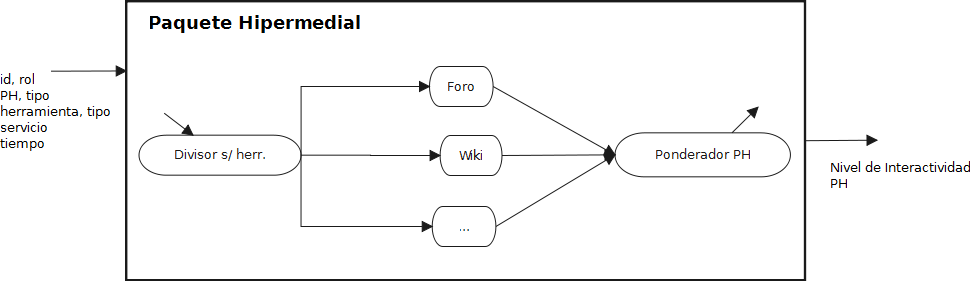
\includegraphics[scale=0.4]{Ch7/f1Dev}
 % .: 0x0 pixel, 0dpi, nanxnan cm, bb=
 \caption{..}\label{}
\end{center}


Fig. 1. Esquema de los módulos acoplados que se integran en un PH.

Y si pensamos que los Paquetes Hipermediales son los componentes conceptuales básicos del Dispositivo Hipermedial Dinámico debemos integrarlos para obtener el nivel total de interactividad de cada participación. La siguiente figura 2 nos muestra el esquema completo:

\begin{center}
 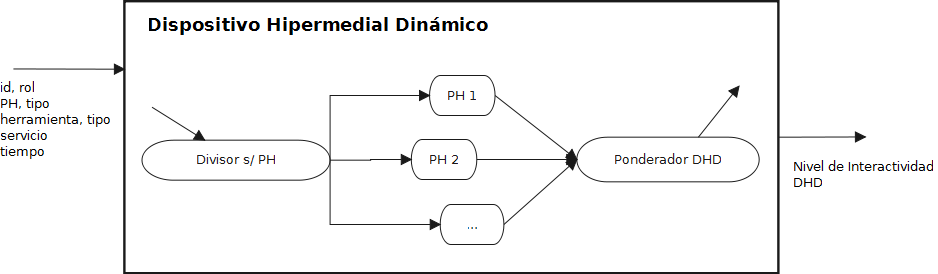
\includegraphics[scale=0.4]{Ch7/f2Dev}
 % .: 0x0 pixel, 0dpi, nanxnan cm, bb=
  \caption{..}\label{}
\end{center}

\caption{Esquema de los módulos acoplados que se integran en un DHD.}



De esta manera se desprende que la información necesaria en nuestro caso es función de las interacciones de los participantes, las cuales estarán definidas por: id del participante, rol del mismo, Paquete Hipermedial sobre el cual participa, tipo de PH, herramienta sobre la cual realiza la interacción, tipo de herramienta, servicio con el cual interactua y el tiempo, día y hora de la interacción.

La fase siguiente corresponde al diseño e implementación de la medición. Este módulo trata con la definición de las métricas que serán útiles para cuantificar los atributos, que en la etapa anterior se identificaron como parte de la especificación de requerimientos, y que son de especial interés en el proyecto, dado que constituyen las características que se medirán para el ente a evaluar, considerando la necesidad de información establecida. Es decir, el objetivo final de la evaluación, que en nuestro caso es el nivel de interactividad de la participación.


De ambas figuras 1 y 2 entendemos la necesidad de plantear tres niveles de métricas para el análisis de las interacciones en tiempo real, dado que nos encontramos con tres entidades diferentes: la herramienta, el ponderador de los PH y el ponderador del DHD.
Es fundamental comprender en el concepto de métrica, qué atributos se cuantifican y a qué entes los asociamos. Asimismo, es preciso identificar el tipo de valor que se obtiene, la unidad en la que se expresa y el tipo de escala que se usa, con el fin de poder realizar una apropiada interpretación y un análisis matemático y/o estadístico.
Siguiendo con las recomendaciones del modelo INCAMI con el propósito de obtener valores para los indicadores globales, debemos tener en cuenta un modelo de acumulación y criterios de decisión. El modelo de ponderación y acumulación (agrupamiento) persigue la confección  de un proceso de evaluación bien estructurado, objetivo y comprensivo para los evaluadores (o la evaluación en sí misma). Al igual que en otros casos de estudio [9], se usaron pesos, modelos de puntuación multi-criterio (consenso)  para designar y ajustar procesos. Un modelo de ponderación (o puntuación) multi-criterio (o por consenso) como LSP, por Logic Scoring of Preference [11], en conjunción con propiedades de sincronización, neutralidad, reemplazabilidad y otras relaciones usando el agregado de operaciones basadas en el modelo matemático de pesos.
El principal objetivo de la implementación de la evaluación global permite mayores niveles de flexibilización para los valores de los indicadores globales y parciales, a partir de los valores de indicadores elementales utilizando el modelo de agrupamiento obtenido para efectuar el cálculo. En este proceso, dichos valores deben ser acordados y consensuados por expertos con experiencia en el uso de este tipo de sistemas. A su vez mencionamos, que los valores numéricos indicados solo buscan mostrar un ejemplo de aplicación. Desarrollos posteriores posibilitarán el responsable de la evaluación pueda dar valor a los diversos coeficientes subrayando aquel atributo que considere más importante en el proceso. En cada caso, el valor resultado brinda una medida sobre el grado de interactividad de la participación.

Métrica de la herramienta

\begin{verbatim}
 

Se construye por un producto de cuatro coeficientes:
	Nivel de interactividad de la participación en la H = C1*C2*C3*C4
Esos cuatro coeficientes estarán en relación a:
Tipo de herramienta
	De formato  trasmisivo (ej.: links, recursos). C1 = 1
	De formato interactivo (ej.: foros, wiki). C1 = 2
Tipo de servicio utilizado
	Crear. C2 = 2
	Consultar. C2 = 1
	Editar. C2 = 2
	Borrar. C2 = 1
Rol del participante
	Docentes. C3 =1
	Alumnos. C3 = 2
Usuarios que utilizan la herramienta
	Uno o dos participantes. C4 = 1
	Tres o más participantes. C4 = 2

Métrica del ponderador del PH
Se construye por un producto de tres coeficientes:
	Nivel Interactividad de la participación en el PH = B1*B2*B3
El valor de estos tres coeficientes serán:
Nivel Interactividad de la participación en la herramienta
	B1 = C1*C2*C3*C4
Tiempo entre la última participación y la actual
	Si es menos de un día. B2 = 3
	Si es menos de una semana. B2 = 2
	Si es más de una semana. B2 = 1
Intercalación entre las herramientas utilizadas
	Si utiliza tres o más herramientas. B3 = 3
	Si utiliza dos. B3 = 2
	Si utiliza una. B3 = 1


\end{verbatim} 


Métrica del ponderador del DHD


\begin{verbatim} 
 
La existencia de diversos tipos de PH (cursos y proyectos en entornos colaborativos, repositorios digitales, Redes Sociales, etc.), con diversas funcionalidades configuradas tanto en sus herramientas, como en sus servicios vinculados, nos habla de la necesidad de ponderar el valor obtenido de la métrica anterior, a fin de normalizar los valores de interactividad de la participación a nivel DHD. 
De esta forma obtenemos:
	Nivel Interactividad de la participación en el DHD = A1*A2
El valor de estos dos coeficientes será:
Nivel Interactividad de la participación en el PH
	A1 = B1*B2*B3
Tipo de Paquete Hipermedial
	Si es un curso. A2 = 1
	Tomando otros valores según el tipo de PH.
\end{verbatim}


Finalmente, en la etapa de evaluación, estas métricas deben ser interpretadas a través de indicadores con el objetivo de evaluar o estimar el grado de conformidad que los requerimientos propuestos alcanzaron. Es en este momento cuando deben seleccionarse los indicadores que interpretarán cada métrica que cuantifica a cada atributo correspondiente en el diseño de los requerimientos no funcionales. Los indicadores contienen también una escala y una función o algoritmo a través del cual será posible interpretar el valor de la métrica, con ayuda también de un criterio de decisión, que establecerá umbrales de aceptabilidad al valor obtenido.


\subsection{Integración en el modelo DEVS}  

Continuando en la línea de la sección anterior, incorporamos las métricas en el modelo original DEVS, para potenciar el análisis de los procesos de educar, investigar, producir y gestionar, y posibilitar un posterior indicador para el cambio contextual de los participantes.
De manera general un modelo DEVS atómico queda definido por la siguiente estructura:


\begin{verbatim}
 

M = (X, Y, S, δint, δext, λ, ta)
donde:
	X es el conjunto de valores de eventos de entrada.
	Y es el conjunto de valores de eventos de salida.
	S es el conjunto de valores de estado.
	δint, δext, λ y ta son funciones que definen la dinámica del sistema.
 
\end{verbatim}

En nuestro caso, el valor de ta, avance de tiempo, que señala el tiempo en que el sistema permanecerá en un estado determinado en ausencia de eventos de entrada, valdrá infinito. Por tanto, δint, la función de transición interna, que recalcula el valor de estado del sistema cuando transcurre el tiempo ta, no es necesario definirla.

Para el caso una herramienta genérica (Foro, Wiki, Blog, etc.):
X: conjunto constituido por las interacciones de los participantes y es un vector de ocho componentes que incluye: id del participante, rol del mismo, Paquete Hipermedial sobre el cual participa, tipo de PH, herramienta sobre la cual realiza la interacción, tipo de herramienta, servicio con el cual interactua y el tiempo, día y hora de la interacción.

Y: conjunto de valores que incluye (vector de nueve componentes): el nivel de interactividad en la herramienta, más el vector anterior.

S: estará determinado por el conjunto de valores de niveles de interactividad a partir de la métrica utilizada por la función de transición externa. 

δext, función de transición externa: aquí es donde insertaremos la métrica para la herramienta expuesta en el apartado anterior.
λ, función de salida: nos devolverá el valor de estado del sistema, es decir el nivel de interactividad de la participación analizada.

En la figura 1 vemos que el PH integra los modelos atómicos de las herramientas y suma a su vez dos módulos atómicos adicionales. El primero que denominaremos divisor PH, será el encargado de redireccionar los eventos a cada herramienta particular. Y el ponderador PH, el cual nos dará el valor global de interactividad del PH a partir del grado de interactividad de cada herramienta y la ponderación.

Para el divisor PH:

X: conjunto de valores de las interacciones de los participantes determinadas por (ocho componentes):  id del participante, rol del mismo, Paquete Hipermedial sobre el cual participa, tipo de PH, herramienta sobre la cual realiza la interacción, tipo de herramienta, servicio con el cual interactua y el tiempo, día y hora de la interacción.

Y: será el mismo evento de entrada, es decir el vector de ocho componentes, pero por el puerto correspondiente a la herramienta solicitada.

S: corresponderá al valor de las componentes del vector del evento de entrada.
δext, función de transición externa: tomará el valor del evento de entrada y a partir del valor del quinto componente definirá el puerto de salida.

λ, función de salida: devolverá el valor actual del estado del sistema, redireccionándolo por el puerto calculado en la función de transición externa.
Para el ponderador PH:

X: el conjunto de valores de entrada coincidirá con los valores de salida de la herramienta (nueve componentes): nivel de interactividad de la participación en H, id del participante, rol del mismo, Paquete Hipermedial sobre el cual participa, tipo de PH, herramienta sobre la cual realiza la interacción, tipo de herramienta, servicio con el cual interactua y el tiempo, día y hora de la interacción.

Y: nos devolverá en un vector de diez componentes: el nivel de interacción de la participación en el PH, más el evento de entrada.

S: estará determinado por el conjunto de valores de niveles de interactividad a partir de la métrica utilizada por la función de transición externa. 

δext: tomará el valor del evento de entrada, nivel de interactividad de la herramienta y lo ponderará a partir de la métrica para el PH expuesta en el apartado anterior.

λ: devolverá el valor de estado calculado en la función de transición externa.

En la figura 2 vemos que el DHD integra los PH y suma a su vez dos módulos atómicos adicionales. El primero que denominaremos divisor DHD, será el encargado de redireccionar los eventos a cada PH perteneciente al DHD. Y el ponderador DHD, el cual nos dará el valor global de interactividad del DHD a partir del grado de interactividad de cada PH y la ponderación.

Para el divisor DHD:

X: conjunto de valores de las interacciones de los participantes determinadas por (ocho componentes): id del participante, rol del mismo, Paquete Hipermedial sobre el cual participa, tipo de PH, herramienta sobre la cual realiza la interacción, tipo de herramienta, servicio con el cual interactua y el tiempo, día y hora de la interacción.

Y: será el mismo evento de entrada, es decir el vector de ocho componentes, pero por el puerto correspondiente al PH de interacción.

S: corresponderá al valor de las componentes del vector del evento de entrada.
δext, función de transición externa: tomará el valor del evento de entrada y a partir del valor del tercer componente definirá el puerto de salida.

λ, función de salida: estará en función del valor actual del estado del sistema, redireccionándolo por el puerto calculado en la función de transición externa.
Para el ponderador DHD:

X: el conjunto de valores de entrada coincidirá con los valores de salida del PH (diez componentes): nivel de interactividad de la participación en el PH, nivel de interactividad de la participación en H, id del participante, rol del mismo, Paquete Hipermedial sobre el cual participa, tipo de PH, herramienta sobre la cual realiza la interacción, tipo de herramienta, servicio con el cual interactua y el tiempo, día y hora de la interacción.

Y: nos devolverá un vector de once componentes: nivel de interacción de la participación en el DHD, más el vector anterior.

S: estará determinado por el conjunto de valores de niveles de interactividad a partir de la métrica utilizada por la función de transición externa. 

δext: tomará el valor del evento de entrada, nivel de interactividad del PH y lo ponderará a partir de la métrica para el DHD expuesta en el apartado anterior.

λ: devolverá el valor de estado calculado en la función de transición externa.



\subsubsection {Condicionales para la coordinación de contratos}

Ahora a tavés de un diagrama UML se definen  las clases utilizadas en la implementación de los Condicionales DEVS dentro de las  reglas de los contractos,   donde se mantienen las propiedades e influencias (relaciones entre elementos conceptuales) descriptas en la figura 1 .

La  figura 2  describe los elementos y relaciones relevantes en la creación de condicionales inferidos por métricas de interacción (sección 4) implementadas en un modelo de simulación DEVS integrado (sección 3). 

\begin{center}
 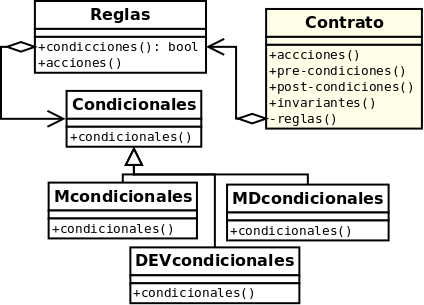
\includegraphics [width=1\linewidth] {Ch7/DEVSCondicional}
 % DEVSCondicional.png: 424x305 pixel, 51dpi, 21.20x15.25 cm, bb=0 0 601 432
 \label{fig:}
 \
\end{center}

Partiendo de una de las propiedades de las reglas  de los contratos sobre la posibilidad de definir comportamiento a través de parámetros context-aware (sección xxx)  e inducidos por reglas donde se designan partes de las  acciones del contrato. De esta manera, las reglas forman parte de un mecanismos de agregación encargado de la composición de diferentes tipos de condicionales, en los que se encuentran  una
familia de condicionales (Condicionales DEVS) conectados a los métodos que implementan las métricas definidas particularmente para la simulación de interacciones (sección xxxx). Las otras dos familias de condicionales representadas por las clases Mcondicionales y MDcondicionales se comportan de manera similares teniendo en cuento el mismo modelo de integración propuesto [cacic 2007]

A continuación se describe los  aspectos principales que se tuvieron en cuenta en la integración de los anteriores sistemas de coordinación de contratos sensibles al contexto y extensiones de condicional para la aplicación de un nuevo sistema de métricas  de interacciones Sakai mediante un modelo de simulación DEVS. 


\subsubsection {Modelo conceptual de integración}

Para implementar la invocación de métricas mediante métodos correctos, propusimos  desde la perspectiva del rediseño e implementación computacional, un modelo de integración de muy bajo costo, sin cambios sustanciales ni en la arquitectura original  ni en el código de la implementación dentro de la aplicación modificada en el proceso de inyección de las propiedades de coordinación de contratos sensibles al contexto [jornal de la clei].

El modelo conceptual de métrica pertenece al Modelo INCAMI (Information Need, Concept model, Attribute, Metric and Indicador: Información relevante, Modelo Conceptual, Atributos, Métricas e Indicadores) (Olsina, L., G. Lafuente y G. Rossi, 2000). INCAMI es un framework organizacional, orientado a la medición y evaluación que permite economizar consistentemente, no sólo metadata de métricas e indicadores, sino también valores mensurables en contextos físicos.

Por medio de un diagrama UML, se representa un modelo general de integración, teniendo en cuenta experiencias vinculadas al agregado de nuevas componentes en determinadas implementaciones resueltas para sistemas Elearning similares al diseño del framework Sakai \cite{libro}. La integración se produce mediante la conexión de las reglas, a través de sus condicionales, con una métrica representada con un método. A su vez,  la métrica es interpretada por un modelo DEVS diseñado para devolver valores de simulación \cite{poner paper de la jaiio o algo parecido a eso}.

\begin{figure} [ht]
\begin{center}
 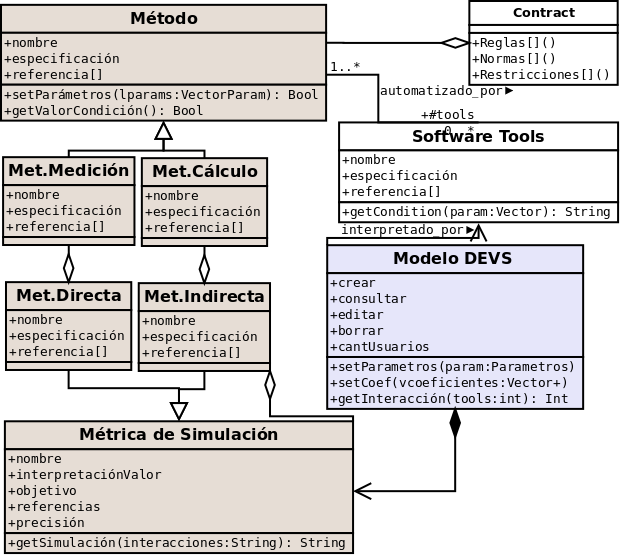
\includegraphics[scale=0.4]{Ch7/I.png}
 % IntegracionDEVScondicional.png: 620x555 pixel, 51dpi, 31.00x27.75 cm, bb=
  \caption{..}\label{}
\end{center}
\end{figure}


En la figura 3 se puede observar lo correspondiente a cada una de las áreas mencionadas, representada con colores diferentes. Además, se muestra que la principal componente para lograr la integración está representada por la incorporación de una relación de agregación entre la componente contrato y la entidad método. Los condicionales de las reglas de los contratos son invocados (mediante un método explícito relacionado con la noción de los Condicionales DEVS, por ejemplo, getForum\_theme) por medio de un mecanismo de callback que permite la correcta invocación de la métrica. 

\\
... completar lo que falta ...
\\

La integración de la métrica con el modelo DEV se produce mediante una vinculación de composición a través de una interfase que permite configurar parámetros de entradas (en este caso: crear, consultar, editar, borrar, catUsuarios ) descripto en los bloques DEVS que representan las métricas implementadas con las interfases descriptas por la clase Métricas de Simulación. El método setCoef  permite establecer las ponderaciones de los los coeficientes que intervienen en la métrica (sección 4); el método setParametros representa todos los parámetros necesarios en la configuración de las herramientas que interpretan modelos DEVS, en este trabajo se usó  PowerDEVS [ref PowerDEV]. Luego, el método getInteracción se encarga de obtener un valor numéro entero representando en nivel de interacción relacionada al parámetro tools  encargado de referenciar a una herramienta del framework Sakai (ej, Foro, Wiki, etc.) que a su ves es representada también con un número entero diferente para cada herramienta. 

La interpretación y manipulación de los resultados de interacciones resueltos en el Modelo DEVS es manipulado por una herramienta de software representada por la clase Herramienta Sakai [herramienta Sakai].  A su vez, por medio de callback desde el Método de la métrica se obtienen  valores para configurar el condicional definitivo para el contrato a través del método getCondición publicado por la Herraminta Sakai.

....
Hablar un poco sobre la herramienta de las coreanas. 
....


\subsubsection {Implementación en un caso de uso}   \label{implementación_en_un_caso_de_uso}

Atendiendo a lo expuesto, seguidamente se implementan lo explicado en el entorno PowerDEVS [12]. El caso de uso fue desarrollado utilizando como punto de partida los Registros de Actividad de Moodle correspondientes a la implementación de una asignatura de grado del Campus Virtual de la UNR [13].

Cada métrica directa tiene asociado un método de medición claramente especificado. Las colecciones de datos son capturados desde la bases de datos (en este caso MySQL). Luego los datos son formateados según la necesidad explicitada en la sección anterior para posibilitar su lectura desde el entorno.

En la figura 3 comparamos los resultados obtenidos de Nivel de Interactividad para cada participación a través del tiempo, en los meses de Agosto/Septiembre (izquierda) y de Noviembre/Diciembre (derecha) para un curso seleccionado en el 2009.

\begin{center}
 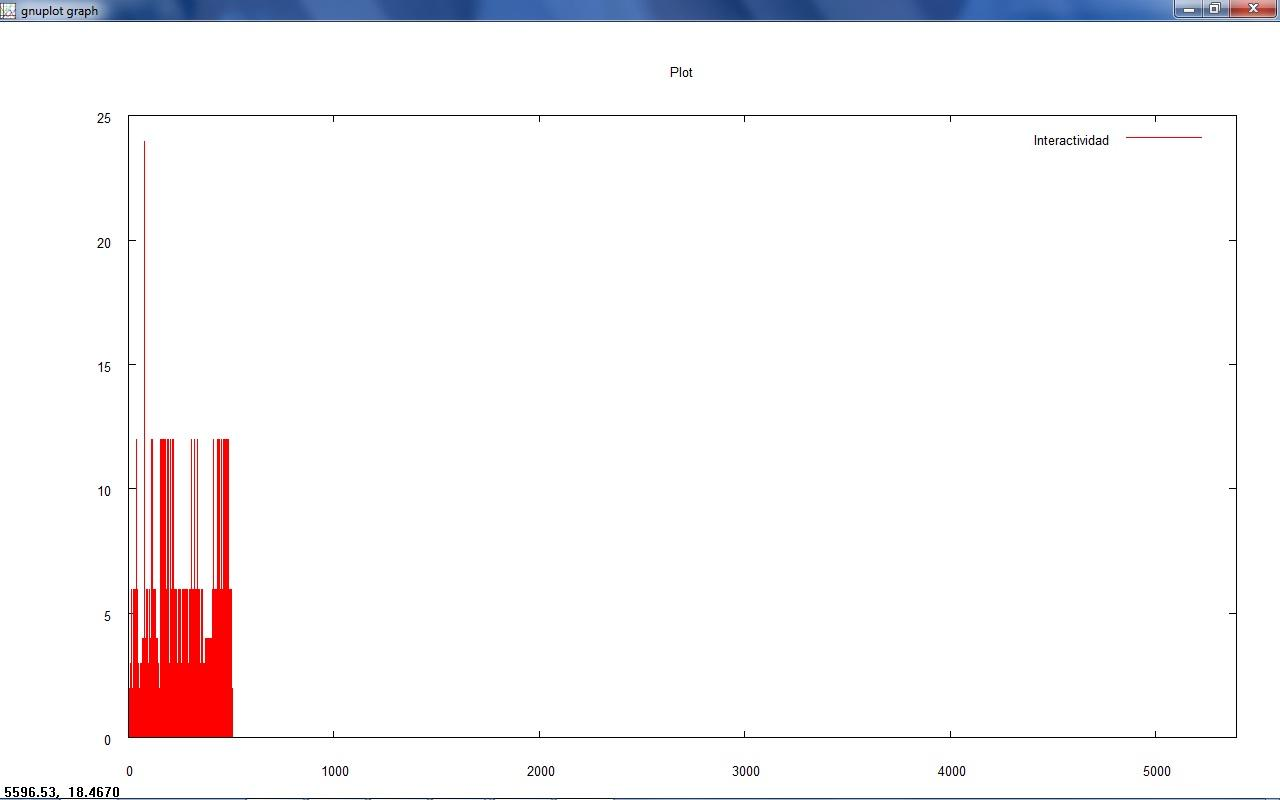
\includegraphics[scale=0.3]{Ch7/f3Dev}
  \caption{..}\label{}
 % .: 0x0 pixel, 0dpi, nanxnan cm, bb=
\end{center}

\caption {Resultados obtenidos en el entorno PowerDEVS} 

Cabe mencionar que los resultados obtenidos son los globales del DHD, pero que sin embargo se disponen a su vez, los valores parciales tanto a nivel Paquete Hipermedial, como a nivel Herramienta individual, (por cuestiones de espacio no mostramos aquí dichos gráficos). Los mismos se exportan a un archivo que relaciona el número de participación, con su nivel de interactividad. Podemos ver en la Figura 4, el seguimiento global del curso mostrando la cantidad de interacciones totales dividida en cada nivel para los meses de Agosto-Septiembre y luego para los meses de Noviembre-Diciembre.
De esta manera podemos observar como se va construyendo la modalidad participativa del DHD a través del crecimiento global de las interacciones (de 505 a 5394), teniendo como valor agregado más allá de la cantidad, las distribuciones de las mismas. Se verifica entonces en los dos últimos meses un 88\% de interacciones en niveles más participativos, en contraposición al 8% de agosto-setiembre. 

\begin{center}
 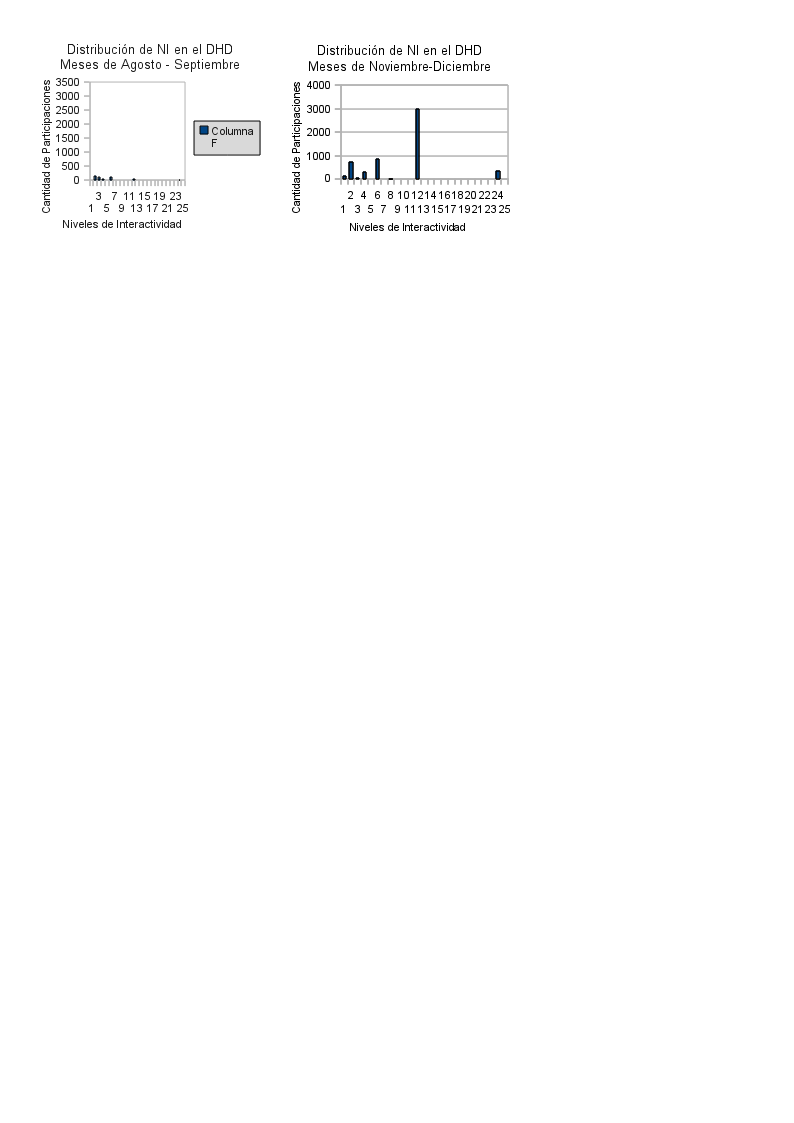
\includegraphics [scale=1] {Ch7/f6Dev}
  \caption{..}\label{}
 % .: 0x0 pixel, 0dpi, nanxnan cm, bb=
\end{center}


\caption {Postproceso de los resultados}

Cabe mencionar que en el ejemplo presentado, los docentes propusieron estrategias didácticas específicas dentro del marco del Programa de Dispositivos Hipermediales Dinámicos que promovían la interactividad responsable para la construcción del conocimiento.

El resultado de este análisis podemos a su vez considerarlo una información de contexto, resignificando una característica del comportamiento de los participantes y atendiendo a la posibilidad de usar la información de interactividad como parámetro context-aware de los contratos [3]. Podremos entonces, establecer un lazo de retroalimentación entre las prácticas efectuadas en los entornos colaborativos, informadas en el Registro de Actividad y las acciones que devengan de los contratos.



\subsection {Consideraciones generales}
  
Fundamentados en el modelado sistémico del DHD, propusimos un primer desarrollo e implementación de métricas para el análisis completo de las interacciones a nivel Herramienta, a nivel Paquete Hipermedial y a nivel Dispositivo Hipermedial Dinámico. Este análisis tiene la versatilidad de estar directamente relacionado según los propósitos de importancia que determinen los sujetos responsables. De esta manera, brindan información calificada y aportan un camino de análisis evaluativo en tiempo real sobre cómo se desarrollan procesos de participación responsable a través de redes sociotécnicas para educar, investigar, gestionar y producir en el actual contexto físico-virtual.


Actualmente nuestros esfuerzos se enfocan al desarrollo de una herramienta de evaluación de espacios físicos-virtuales, integrada y de código abierto, que otorgue mayor flexibilidad y dinamismo a los componentes que pueden configurar al DHD para la construcción y diseminación de conocimiento.
